\chapter*{Ouders en Voorouders}
\lettrine[lines=2, loversize=0.3, lraise=0]{\initfamily M}{ijn }
ouders zijn tegelijkertijd getrouwd met mijn moeders broer, Piet Vlam, en zijn vrouw. 
\begin{figure}[h]
    \begin{centering}
    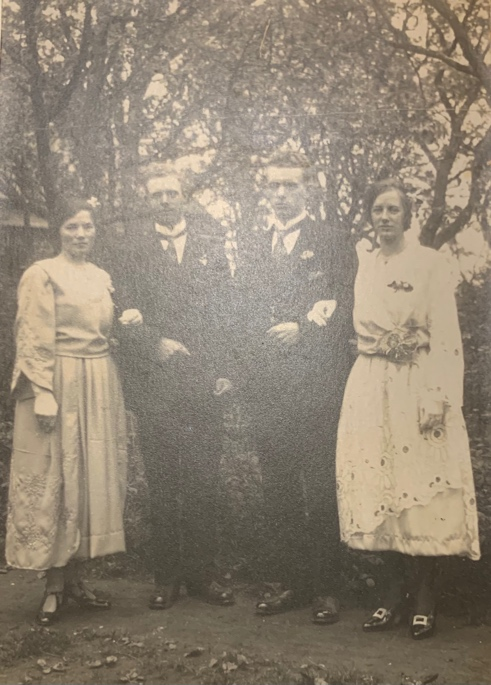
\includegraphics[width=0.5\textwidth]{image11}
    \caption{Zojuist getrouwd.}
    \end{centering}
\end{figure}

Met die broer had ze verder niet veel contact overigens. Ik vond het ook geen leuke man.
Volgens mijn moeder was hij als kind wel leuk maar is hij zo geworden door zijn vrouw. Dat was een beetje een haaiebaai.

\begin{figure}[h]
    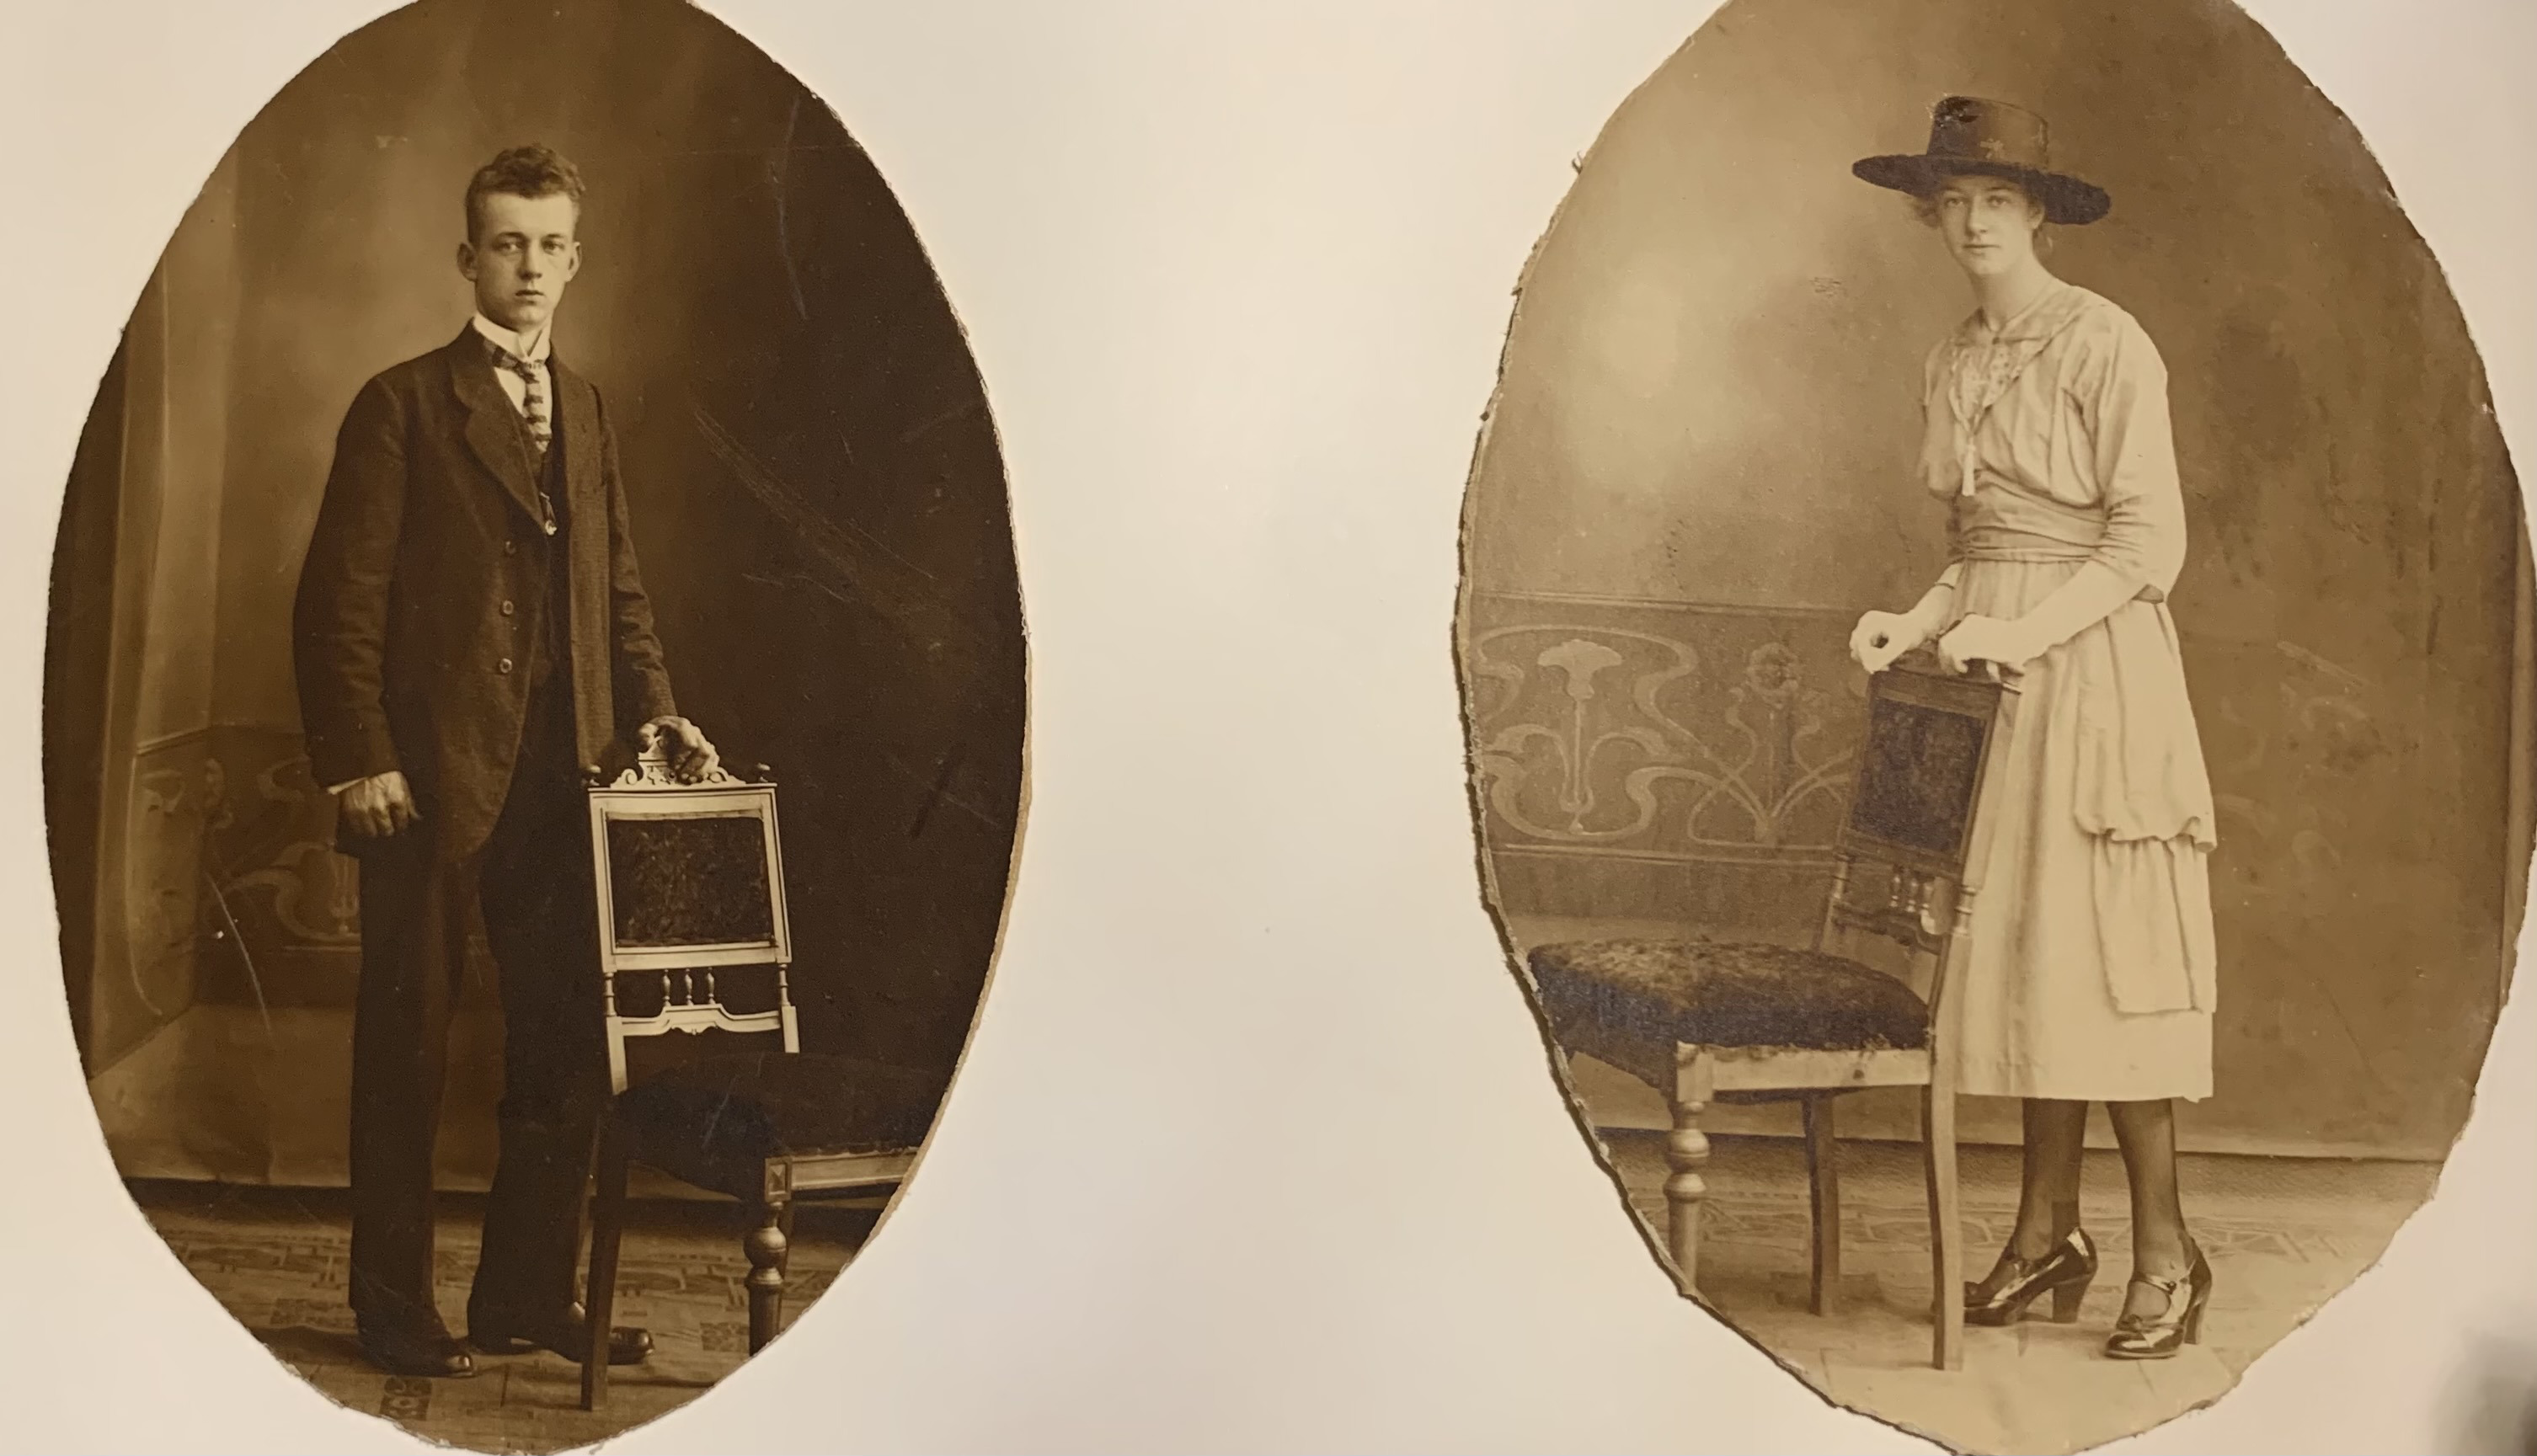
\includegraphics[width=\textwidth]{image12}
    \caption{Mijn ouders.}
\end{figure}

\begin{figure}[h]
    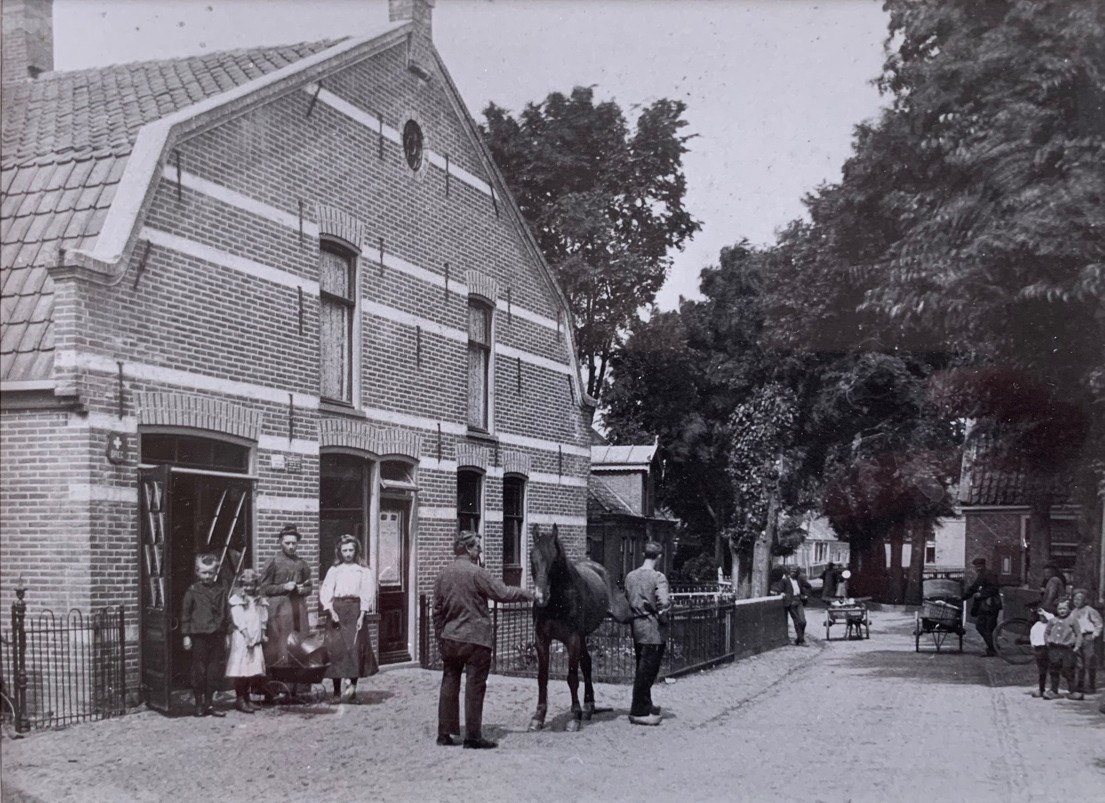
\includegraphics[width=\textwidth]{image13}
    \caption{De smederij; links mijn vader als jongetje, met zijn moeder en zussen. De smid is mijn opa.}
\end{figure}

Mijn vader kwam uit Oudkarspel. Zijn ouders hadden daar de smederij in het huis waarin ik ben geboren. 

Zijn voorouders kwamen allemaal uit Noord-Holland; o.a. uit Enkhuizen. 

Hij had twee zussen. Die heetten Trien en Rentsje.

Hij was ondernemend en goed opgeleid, eerst tot smid, en later heeft hij in Antwerpen nog een opleiding m.b.t. auto’s gevolgd.

In hun verkeringstijd haalde hij mijn moeder op met de motor. Hij was de bink van de streek. Er was toen zo weinig verkeer dat ze hem al van verre hoorde aankomen.

\begin{figure}[h]
    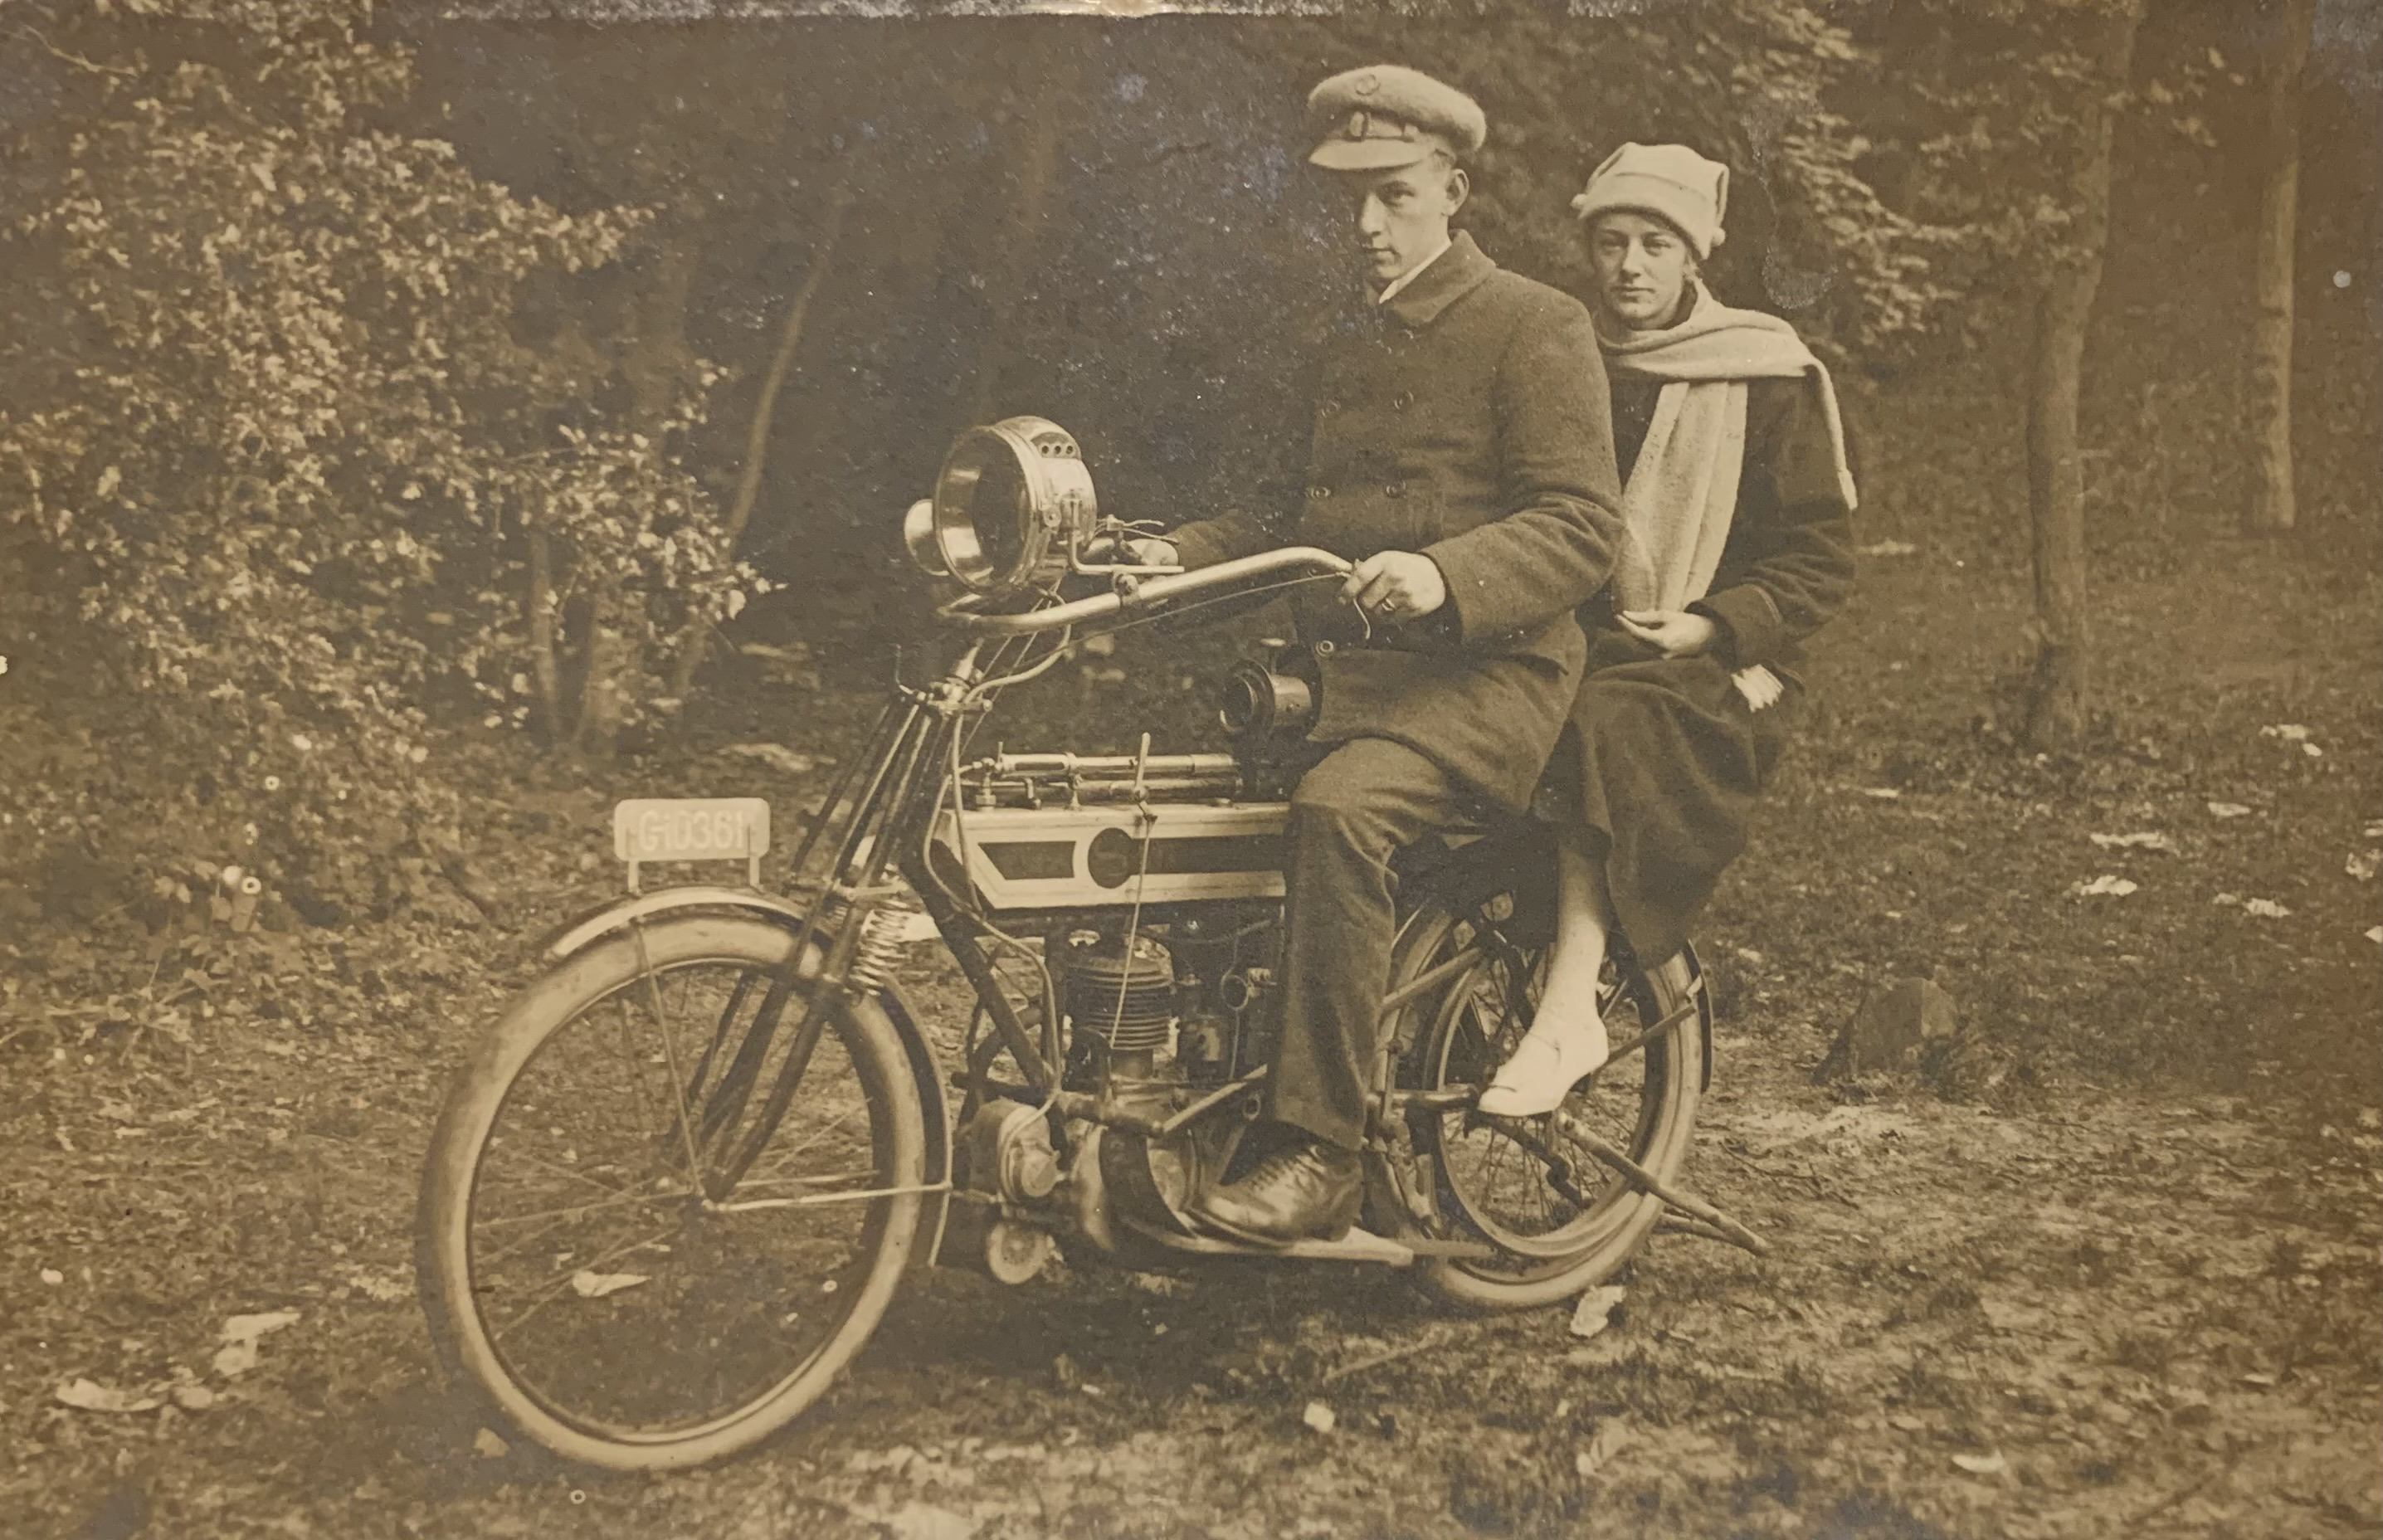
\includegraphics[width=\textwidth]{image14}
    \caption{Mijn ouders in hun verkeringstijd.}
\end{figure}

Mijn moeder was een Vlam uit Schoorldam. Zij had een broer Piet en een oudere zus, Hidda. 

\begin{figure}[h]
    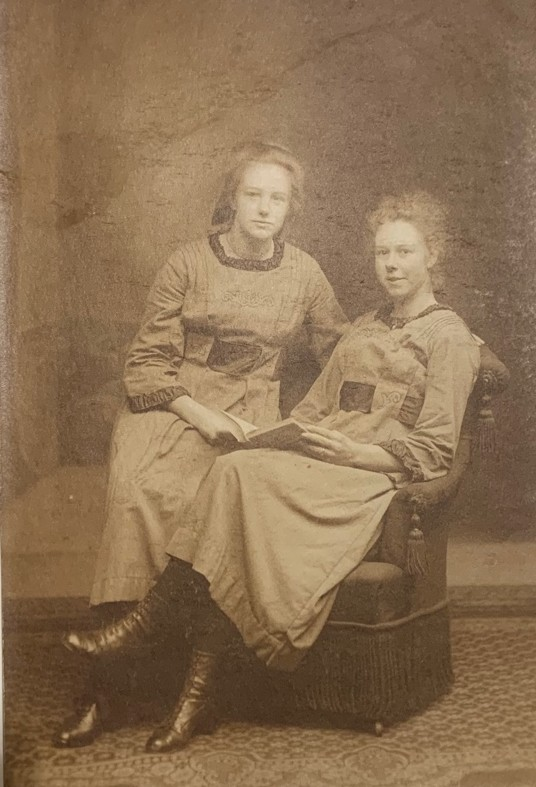
\includegraphics[width=0.8\textwidth]{image15}
    \caption{Mijn moeder (rechts) en haar zusje.}
\end{figure}

\begin{figure}[h]
    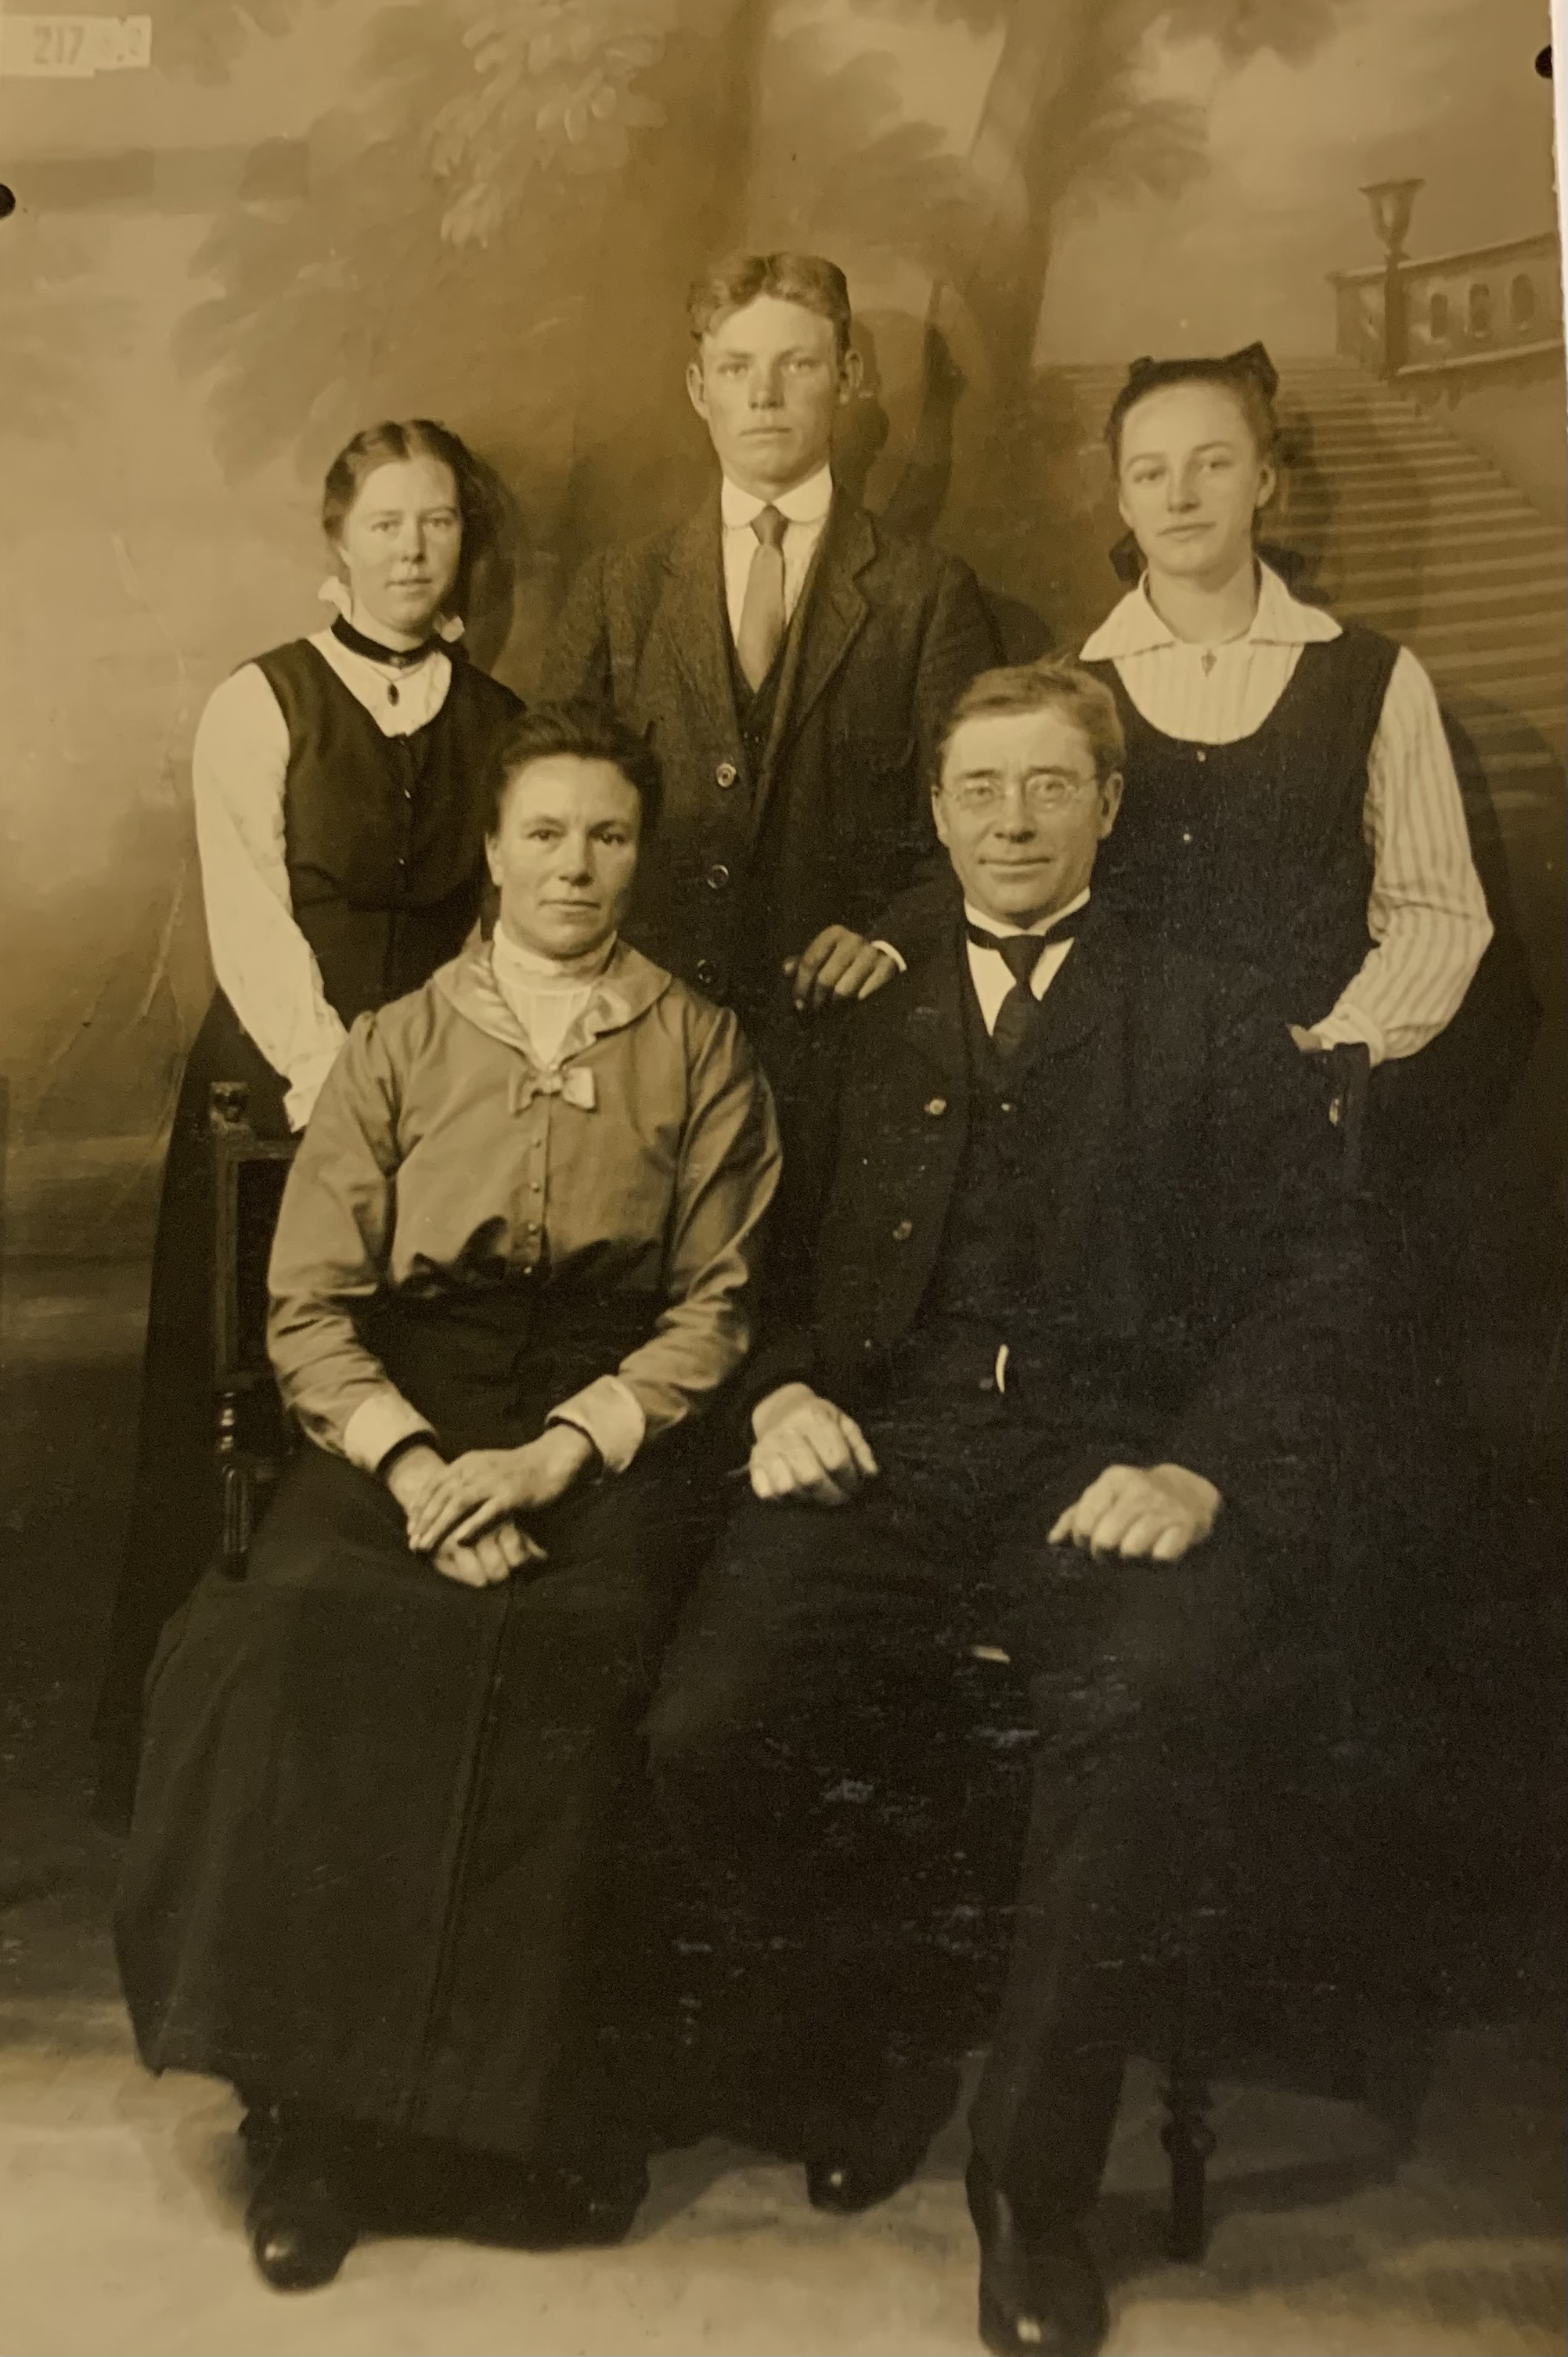
\includegraphics[width=0.9\textwidth]{image16}
    \caption{De familie Vlam (rechts achter mijn moeder).}
\end{figure}

Mijn opa had samen met zijn niet getrouwde broer (ook weer een Piet) een boerderij. 

Mjn opa en oma woonden in een huis aan het Noord-Hollands kanaal. Broer Piet woonde op de boerderij. Voor die tijd was het een grote boer. Als je door het washok liep waren er links en recht stallen, en verderop stallen voor de paarden. En er liep ook een varken rond.

De ouders van mijn moeder hadden de scheepswerf op Schoorldam. Het was een gegoede familie. Later is die werf in handen gekomen van een andere familie. 

\begin{figure}[h]
    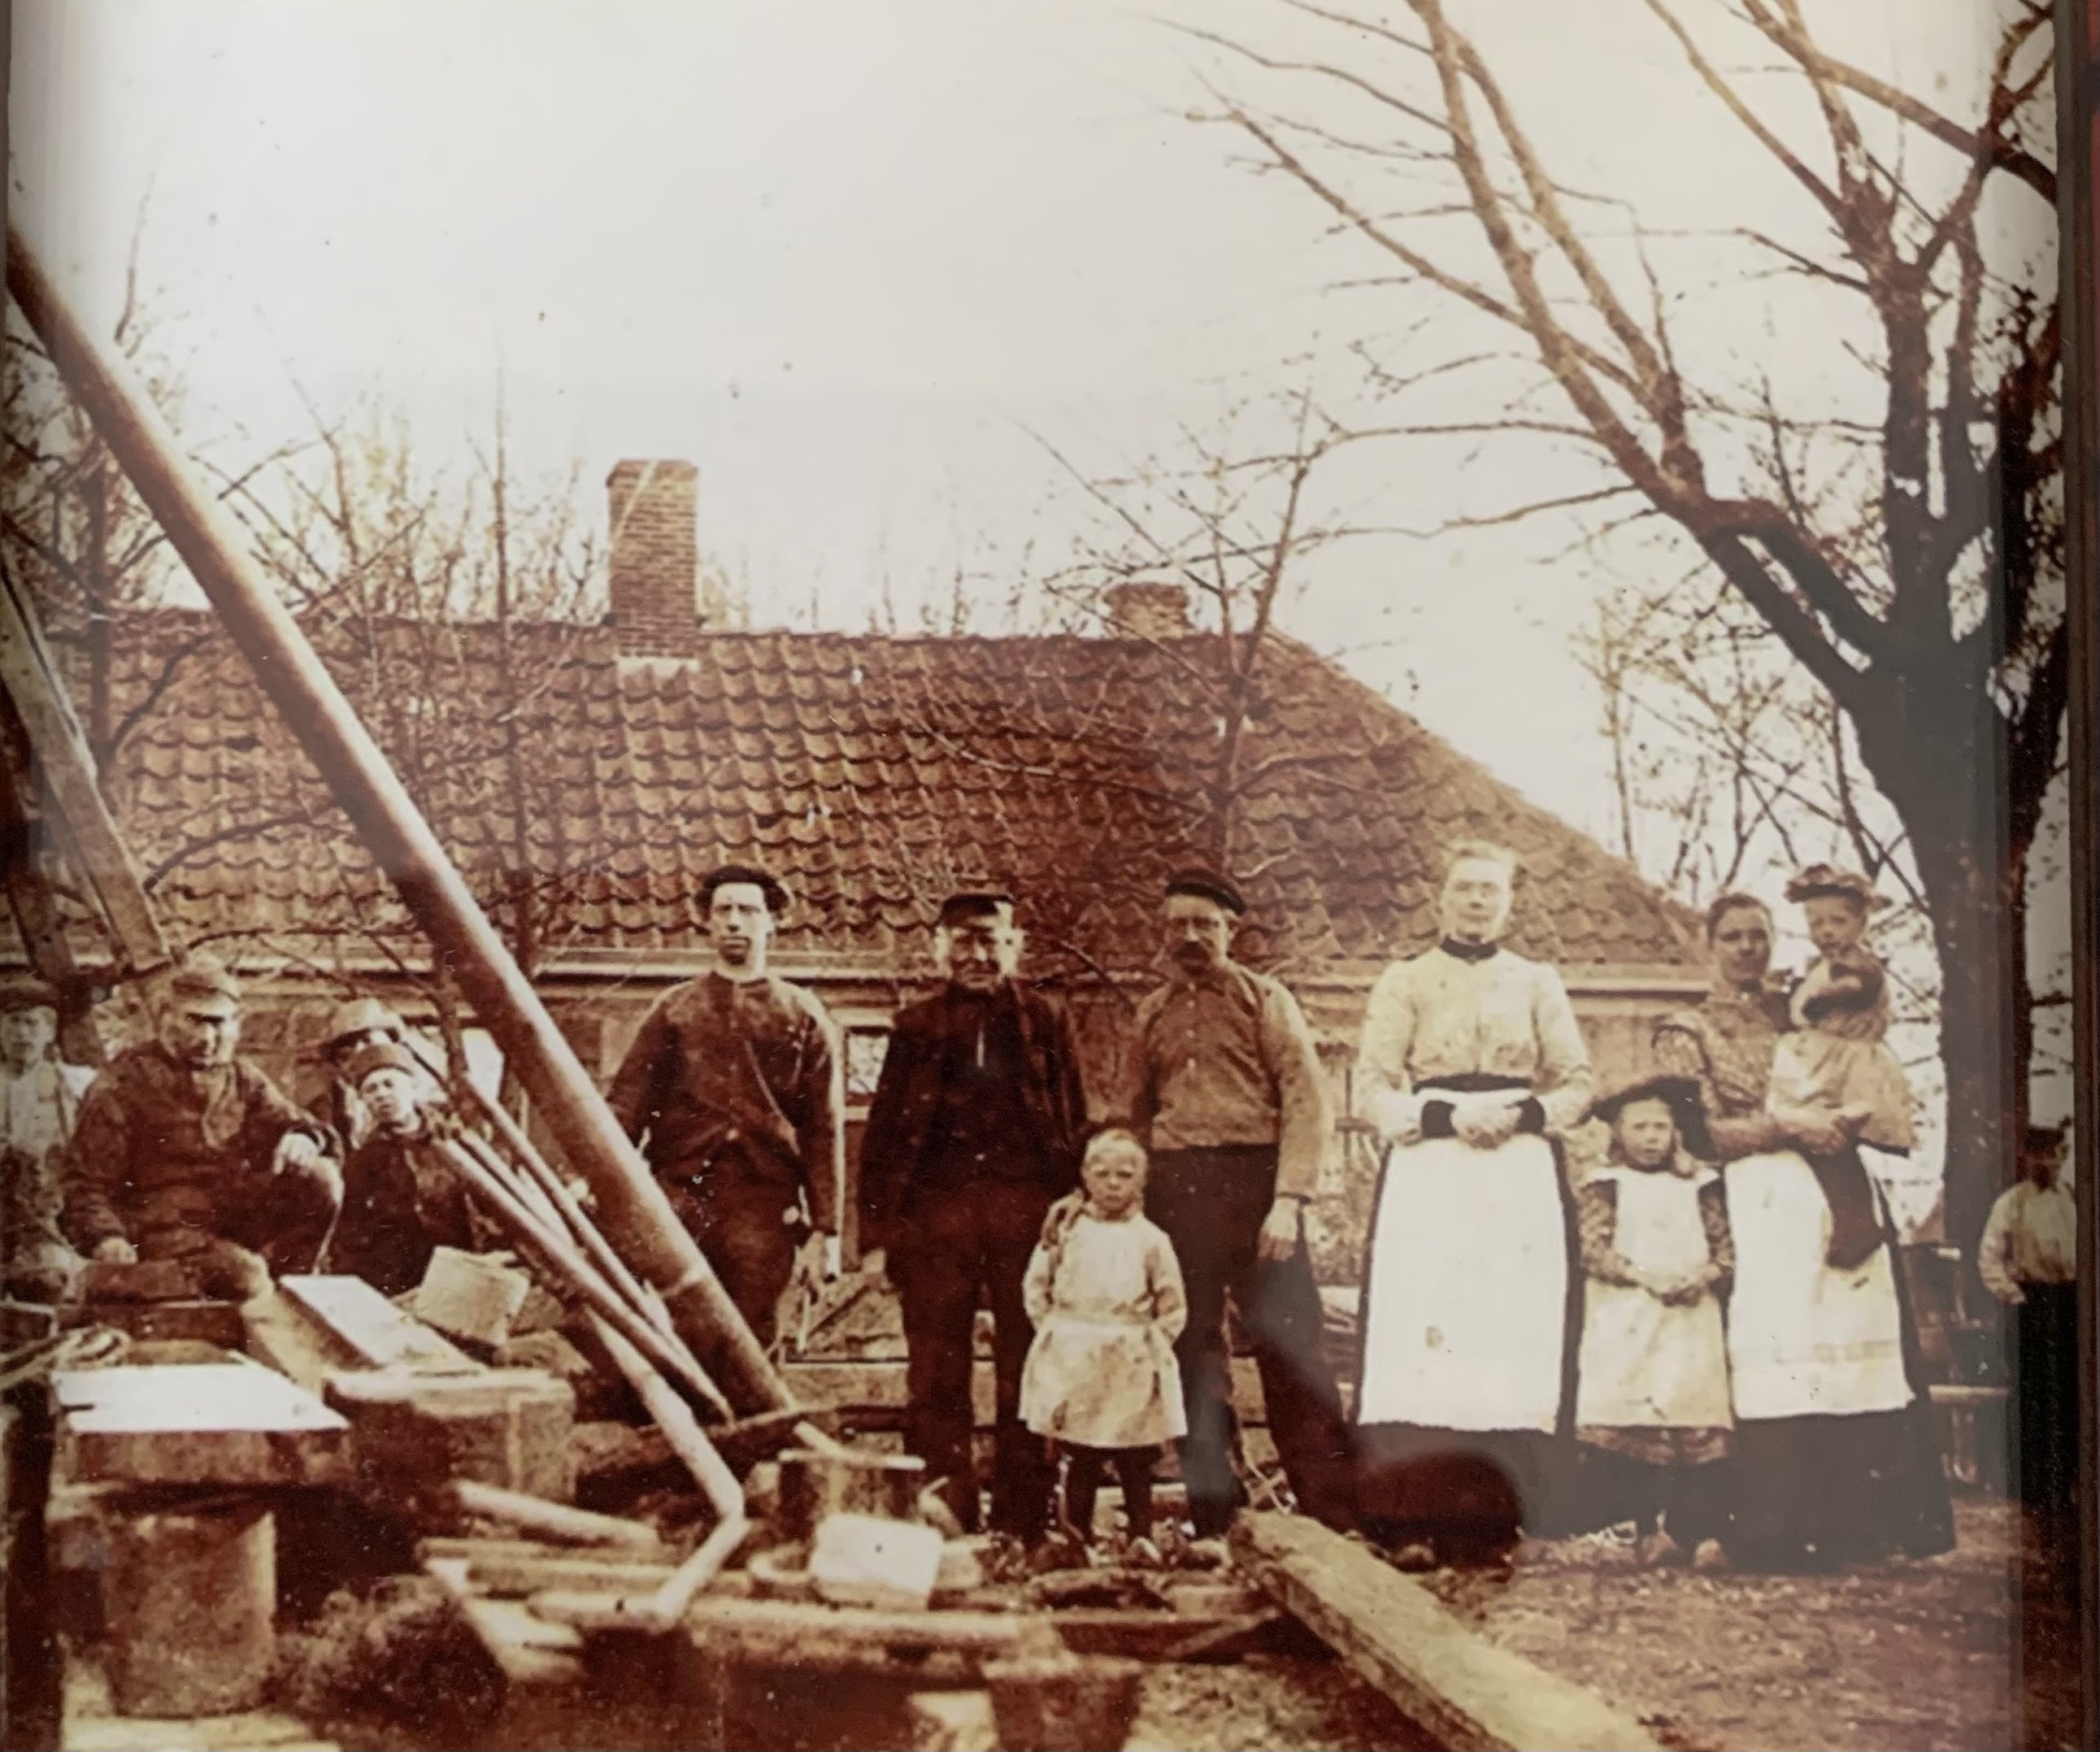
\includegraphics[width=\textwidth]{image17}
    \caption{Bij de werf. Rechts mijn oma met mijn moeder op de arm.}
\end{figure}

De oma van mijn oma kwam uit Friesland, uit Kimswerd. Riemke Jans Westra heette ze, geboren in 1803. Van haar geboorte is de geboortelepel bewaard gebleven. 

Zij kwam met een dominee mee naar Noord-Holland voor een dienstbetrekking. Later heeft ze ook nog in het onderwijs gewerkt dus het moet een slimme vrouw zijn geweest. Ze is overleden in 1873.

\begin{figure}[h]
    \begin{centering}
    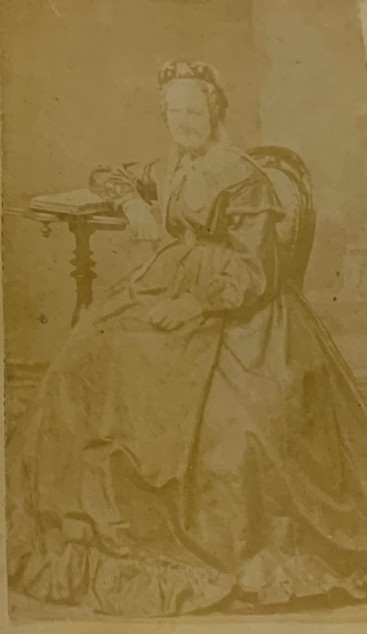
\includegraphics[width=0.7\textwidth]{image18}
    \caption{Riemke Jans Westra (geboren 1803).}
    \end{centering}
\end{figure}

\begin{figure}[h]
    \begin{centering}
    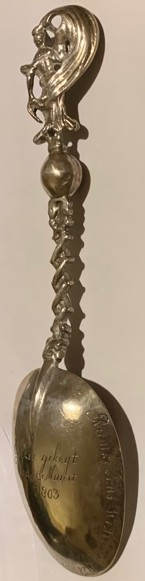
\includegraphics[width=0.3\textwidth]{image19}
    \caption{De geboortelepel die voor Riemke Westra gemaakt is. De inscriptie vermeld dat hij op het ijs van de destijds bevroren Zuiderzee is gekocht.}
    \end{centering}
\end{figure}


\begin{figure}[h]
    \begin{centering}
    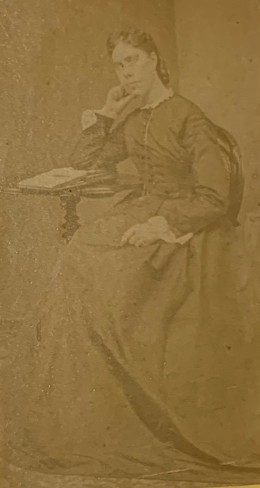
\includegraphics[width=0.7\textwidth]{image20}
    \caption{Hittje (Aaltje) Westra.}
    \end{centering}
\end{figure}

Haar dochter Hittje (die zich Aaltje noemde, ze vond Hittje zeker geen mooi naam; 1830-1950) heeft ook als onderwijzeres gewerkt.

Ik heb een vriendin gehad die ook een Westra was, IJda Westra. Ze was in de verte familie. Haar vader was niet erg aardig voor haar. Haar moeder was wat ziekelijk en toen moest IJda alles maar overnemen. Als ze dan op school kwam had ze al weet ik hoeveel gedaan in het huishouden. Haar vader legde expres iets waar ze bang voor was in de kast waar zij dingen uit moest pakken.

\begin{figure}[h]
    \begin{centering}
    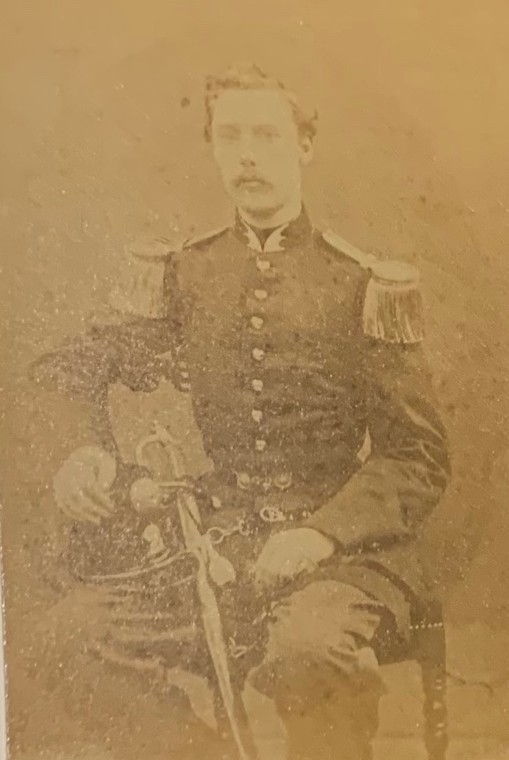
\includegraphics[width=0.7\textwidth]{image21}
    \caption{Jan Vlam, de tekenaar.}
    \end{centering}
\end{figure}

In de familie zijn veel tekeningen bewaarde gebleven. Die zijn gemaakt door Jan Vlam (1833-1890), de broer van Hittje. Hij tekende op alles wat los en vast zat.

\begin{figure}[h]
    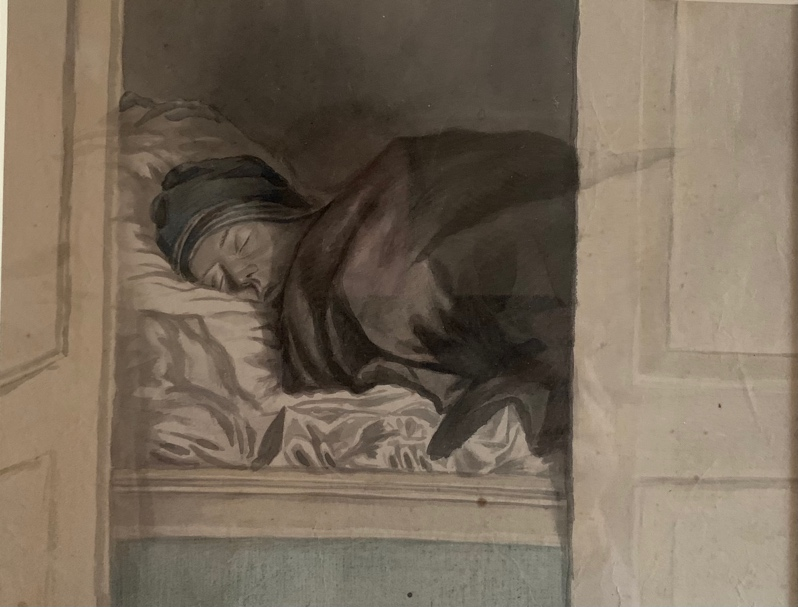
\includegraphics[width=\textwidth]{image22}
    \caption{Jan vlam, tekening van zijn broer Pieter Vlam (1828-1914) in de bedstee. Pieter was de opa van mijn moeder.}
\end{figure}
